\chapter{How to Have an Impactful Role in the Company}

This short lecture answers a practical question by refusing to answer it too quickly. We are asked what the day-to-day work was and what made it impactful, and the speaker replies by rewinding the story until the structure of the role can be seen as a sequence of enlargements: first a narrow commercial post, then the whole customer interface, and finally a move into company operations. There is little literal mathematics here, but there is a clean organizational mechanics, and it is useful to write it in compact form.

\section{The Opening Question}

The question is concrete: what did he do at HMS, and what part of that role mattered most? The answer begins with a retreat in time. Instead of giving a job description, he says, in effect, that we must first recover the path by which the responsibility set grew.

This matters for the notes. The lecture is not organized as a list of duties. It is organized as a sequence of changes in what the speaker was responsible for, and the payoff comes only after those changes have been made visible.

\section{The Initial Boundary of Responsibility}

At the starting point, the bundle is small enough to write explicitly. Let \(R_0\) denote the initial responsibility set:
\begin{equation}
R_0 = \{\text{commercial sales},\ \text{account management}\}.
\end{equation}

\begin{definition}
We shall use \(R\) to denote the set of functions for which the speaker has direct leadership responsibility at a given stage of the story.
\end{definition}

This notation is already helpful, because the transcript is really about boundary changes. Each later step is best understood as an update of \(R\), not merely as a new title. We begin, then, with a sharply bounded commercial role.

\section{Expansion to the Customer Interface}

After about a year, the head of federal and state leaves, and the CEO tells him to take over those areas. The lecture then does something important: it does not stop with the minimal update, but expands the list until the whole customer-side surface becomes visible.

\paragraph{Worked update rule.}
We can write the enlargement in two passes. First comes the explicit addition forced by the vacancy,
\begin{align}
t_{\mathrm{expand}} &\approx 1\ \text{year},\\
R_0^{+} &= R_0 \cup \{\text{state},\ \text{federal}\}.
\end{align}
Then comes the speaker's fuller summary of what he in fact had:
\begin{equation}
R_1 =
\{\text{commercial},\ \text{state},\ \text{federal},\ \text{sales},\ \text{account management},\ \text{marketing},\ \text{government relations}\}.
\end{equation}

The list should be left slightly rough, because it is spoken, not drawn from a formal org chart. In particular, ``commercial'' and ``sales'' may overlap, but the point of the narration is accumulation, not taxonomic tidiness.

\begin{definition}
Let \(R_{\mathrm{cust}}\) denote the bundle of functions that, in the speaker's own phrase, ``touched a customer'' at HMS.
\end{definition}

\begin{equation}
R_1 \approx R_{\mathrm{cust}}.
\end{equation}

This approximation is the first real answer to the opening question. The role becomes impactful not because a title becomes grander, but because the boundary of responsibility expands until it covers the firm's customer-facing interface.

\subsection{Question \& Answer}

\paragraph{Question.}
What actually makes the role impactful at this stage: rank, title, or breadth of responsibility?

\paragraph{Answer.}
The transcript points to breadth. Once the speaker can say that he ran everything at HMS that touched a customer, the role is no longer a narrow commercial post. It has become a control surface for the way the company meets its market.

\section{Scale and Duration}

The lecture does not leave that claim floating. It attaches both a scale and a duration. At the time, HMS was operating at roughly a \$400 million run rate, and this customer-touching role was not a brief emergency assignment.

\begin{align}
\mathrm{RunRate}_{\mathrm{HMS}} &\approx \$400\,\mathrm{M},\\
t_{\mathrm{cust}} &\approx 4\ \text{years}.
\end{align}

These two numbers matter. Scale tells us that the bundle \(R_{\mathrm{cust}}\) was economically consequential, and duration tells us that the arrangement was stable enough to become the speaker's actual working regime rather than a temporary overlap of duties.

\section{From Client-Facing Scope to Operations}

After those four years, the next move is motivated by a problem. One division is under severe challenge, and the speaker asks the CEO to put him in charge of it. This is an important change in the logic of the story: the earlier expansion came from organizational vacancy, while this one comes from a troubled operating unit and a deliberate request to take responsibility.

To make the move possible, someone else is brought in to run the client-facing bundle. The speaker then says that he took over the COB business, the payment integrity business, and the IT shop. We therefore write
\begin{equation}
R_{\mathrm{ops}} = \{\text{COB},\ \text{payment integrity},\ \text{IT}\}.
\end{equation}

The overall sequence can be summarized by a compact transition law:
\begin{equation}
R_0 \xrightarrow{\text{CEO adds state/federal}} R_{\mathrm{cust}}
\xrightarrow{\text{division challenge}+\text{handoff}} R_{\mathrm{ops}}.
\end{equation}

\begin{figure}
\begin{center}
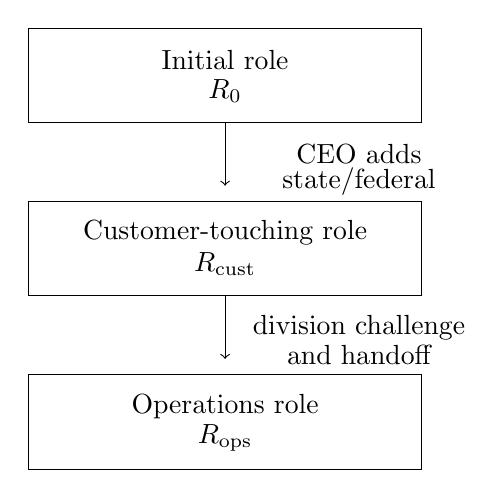
\begin{tikzpicture}[x=1cm,y=1cm]
\draw (0,4.2) rectangle (5,5.4);
\node at (2.5,5.0) {Initial role};
\node at (2.5,4.6) {\(R_0\)};

\draw[->] (2.5,4.2) -- (2.5,3.4);
\node at (4.2,3.8) {CEO adds};
\node at (4.2,3.45) {state/federal};

\draw (0,2.0) rectangle (5,3.2);
\node at (2.5,2.8) {Customer-touching role};
\node at (2.5,2.4) {\(R_{\mathrm{cust}}\)};

\draw[->] (2.5,2.0) -- (2.5,1.2);
\node at (4.2,1.6) {division challenge};
\node at (4.2,1.25) {and handoff};

\draw (0,-0.2) rectangle (5,1.0);
\node at (2.5,0.6) {Operations role};
\node at (2.5,0.2) {\(R_{\mathrm{ops}}\)};
\end{tikzpicture}
\end{center}
\end{figure}

The diagram is only a transcript-based reconstruction, but it captures the lecture's real geometry. The path is not from small job to big job in some generic sense. It is from a narrow customer role, to the whole customer interface, and then into the operating core of the company.

\section{What the Pivot Means}

The last sentence of the excerpt is garbled, but its direction is clear enough to preserve. The speaker is trying to distinguish a fully external-facing role from running operations. We should resist the temptation to repair the wording too aggressively; the safe claim is that impact deepens when responsibility passes from managing contact with the customer to managing the internal machinery that determines whether the firm can perform.

There is also a useful asymmetry between the two expansions. The first makes him responsible for more of what the customer sees. The second makes him responsible for more of what produces the outcome. That is why the story feels like an answer to the original question rather than merely a chronology of promotions.

\section{Summary}

The lecture begins with a question about day-to-day work and turns it into a question about the changing boundary of a role. We start with \(R_0 = \{\text{commercial sales},\ \text{account management}\}\), we move to an approximately customer-complete bundle \(R_{\mathrm{cust}}\) at meaningful scale, and we end with an operating bundle \(R_{\mathrm{ops}}\) that includes COB, payment integrity, and IT. The practical lesson is that impact is narrated here as an increase in scope, leverage, and operating consequence, and the order of that narrative should be kept intact in the final chapter.